\section{Exercice 4}

\begin{enumerate}
      \item
            \q{Définir sous python cette fonction.}\\
            \q{La faire tracer dans l'intervalle $[0, 1]$ par pas de $0.01$ et
                  faire tracer la composée $f(f(f(x)))$.}

            Voici \il{f} :
            \codeFromFile{section-01/q1-1.py}
            Voici sa réciproque :
            \codeFromFile{section-01/q1-2.py}
            Voici composée $n^{\grave{e}me}$ :
            \codeFromFile{section-01/q1-3.py}
            Je trace tout ça :
            \codeFromFile{section-01/q1-4.py}
            Et ça donne :
            \begin{center}
                  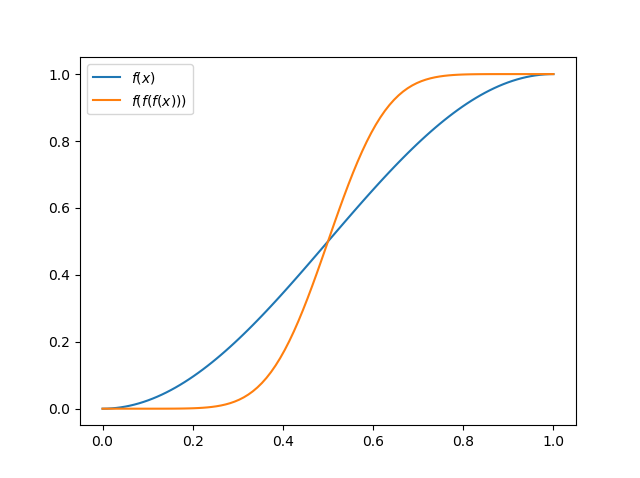
\includegraphics[scale=0.8]{section-01/q1-5.png}
            \end{center}

      \item
            \q{Définir sous python la fonction}
            $g(x) = E(f(f(f(\frac{x}{256})))\times 256)$
            \q{ avec }$E(s)$\q{la partie entière de }$s$.
            Je le fais pour $n$ intération et non seulement 3.
            \codeFromFile{section-01/q2.py}

      \item
            \q{Ecrire le programme permettant de charger l'image en niveau de
                  girs nommée }\il{image_grise.jpg}\q{, de lui appliquer la fonction
                  $g$ et de visualiser cette image.}\\
            Je préfère traiter cette question directement avec la suivante.

      \item
            \q{Comment diminuer le contraste ? Ecrire cette fonction et la tester.}


            \bigskip

            Pour diminuer le contraste, il faut composer plus que 3 fois $f$.
            \bigskip
            Voici la fonction \il{contraste} :
            \bigskip
            \codeFromFile{section-01/q4-1.py}
            \newpage
            On teste :
            \codeFromFile{section-01/q4-2.py}
            Ce qui donne (de gauche à droite \il{c=0}, \il{c=+2}, \il{c=-2}) :
            \begin{center}
                  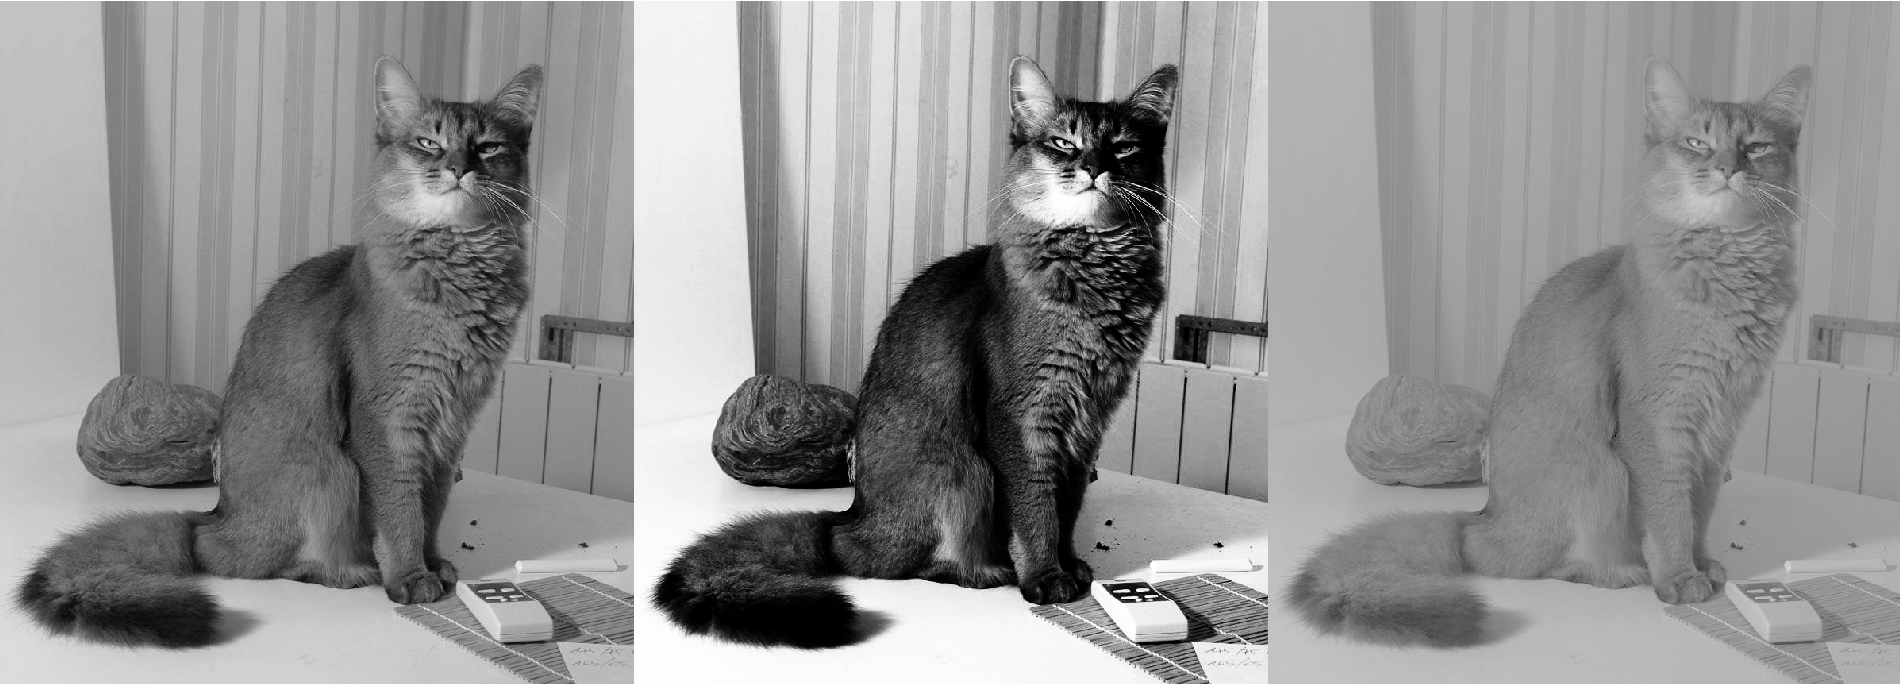
\includegraphics[scale=0.2]{section-01/q4-3.png}
            \end{center}


\end{enumerate}
